Como ya hemos visto, el propósito de un octavador es proporcionar una señal una octava inferior a la señal introducida. En consecuencia el algoritmo debe dividir la frecuencia de cada muestra entrante por dos. Lo primero que salta a la vista es la manifiesta relación con la transformada de Fourier para operar en el dominio de la frecuencia, sin embargo, el coste computacional y temporal de implementar esta operación matemática es elevado. Es por ello que se estudian diferentes posibilidades que pudiesen simplificar la ariquitectura.

\section{Aproximaciones al problema}
El primer pensamiento es que se trata de algo sencillo: basta con eliminar una de cada dos muestras en el espectro, es decir, un diezmado en frecuencia, para obtener a la salida una señal con las frecuencias divididas por dos. Sin embargo las propiedades de la transformación hacen imposible realizar esta operación. Como las frecuencias de entrada son numerosas y variables, no basta este diezmado, ya que el desajuste en la fase produce un desplazamiento circular en la señal de salida (ecuación~\ref{eq:DESP}). 

\begin{equation}
\label{eq:DESP}
Si~~~~~\mathscr{F}(\{x_{n}\})_{k} = X_{k}~~~~~Entonces~~~~~\mathscr{F}(\{x_{n}e^{\frac{2\pi i}{N}nm}\})_{k}= X_{k-m} 
\end{equation}

La consecuencia es que si la señal de entrada no es una única nota invariante, la salida resulta irreconocible, descartando inmediatamente este proceder. [GRAFICA DE LA ENTRADA/SALIDA EN ESTE CASO MATLAB] Otra consideración que no hay que dejar de lado es la pretensión de operar en tiempo real. Esto supone que se debe tener en cuenta un mecanismo que permita trocear la señal en conjuntos finitos para poder aplicar la transformación de Fourier. Este proceso, junto con la propia implementación de la transformada va a complicar en gran medida la arquitectura, es por ello que se decide en primer lugar evaluar los algortimos que no precisan de la esta operativa.

\subsection{Prescindiendo de Fourier}
\label{nofourier}
De cara a obtener un pedal de efectos para un instrumento más grave, se podría haber pensado en optar por un octavador ascendente. Esto, aunque parece que plantea los mismos problemas, resulta mucho más sencillo de implementar precisamente por ser 2 el factor de multiplicación. La fácil solución consiste en elevar cada muestra al cuadrado y realizar un filrado pertinente que aisle las componentes que nos interesan, de forma que $X_{out} = X_{in}^{2}$, según vemos en el gráfico [INSERTAR GRAFIO MATLAB]. Como se puede apreciar, se produce un aumento llamativo de los armónicos produciendo una ligera variación en el timbre que podría resultar interesante, este tipo de efectos recibe el nombre de \emph{ennhancer}\footnote{Esta operativa me fue propuesta por José Parera, al que agradezco mucho el tiempo que me dedicó desinteresadamente} ya que se puede modificar el timbre de forma significativa. Si añadiesemos a este otros efectos como tremolo, reverb o delay, podríamos realizar una aproximación muy válida a un pedal comercial, sin embargo, he preferido mantnerme fiel a la intención original de realizar la octavación descendente.

No obstante, merece la pena probar que ocurre si realizamos la operación opuesta, $X_{out} = \sqrt{X_{in}}$, de forma que se octavara hipotéticamente la señal de forma descendente. EL resultado es menos halagüeño de lo que pudiera parecer, en primer lugar tenemos el inconveniente de tener que lidiar con las muestras de valor negativo\footnote{Como se verá más adelante, el método de entrada en la FPGA devuelve las muestras normalizadas en el rango (-1,1)}, lo que resulta una molestia de cara al flujo de datos. Además, debido a que la entrada está limitada en banda, al reducir de forma cuadrática el valor de los armónicos más agudos, se produce una modificación en el timbre que provoca un sonido \emph{robótico} o \emph{artificial} por lo que se descarta también esta idea.

La última de estas operativas \emph{sencillas} consiste en utilizar las propiedades de la multiplicación por coseno para modular la señal a la altura deseada. Aunque la idea parece sencilla, resulta muy complicado de llevar a la práctica puesto que habría que implemntar un algoritmo que detectara los picos de frecuencia y los modulara utilizando un coseno de valor $f_{pico}/2$. La detección de picos en frecuencia ya supone otra vez la vuelta al dominio de Fourier sin contar con que la gestión de la anchura de esos picos de frecuencia podría suponer una vez más una reconstrucción ininteligible. EL algoritmo de baja frecuencia que se describe posteriormente en la sección~\ref{rhilbert} propone algo similar.

\subsubsection{Algoritmo NFC-TSM}
En este momento descubrí gracias una vez más a la charla con José Parera, la existencia de \emph{dafx.com}, que se trata de una página dónde se publican anualmente un gran número de estudios relacionados con los efectos digitales de audio y de donde he obtenido la mitad de las referencias bibliográficas. De la investigación en esta página descubrí un algoritmo que realizaba la octavación descendente sin llevar a cabo la transformada de Fourier, descrito en \cite{nfctsm}.

Este documento propone un ingenioso algoritmo al que llaman Modificación de Escala Temporal por Correlación Normalizada y Filtrada o por sus siglas en inglés \emph{NFC-TSM}. El funcionamiento es el siguiente; primeramente se lleva a cabo un remuestreo con la tasa deseada $f_{s_original}/f_{s_replay}$ que en el caso de la octava debería ser de 2:1. En segundo lugar tiene lugar el proceso de la modificación de la escala temporal.

\begin{figure}[!ht]
\begin{center}
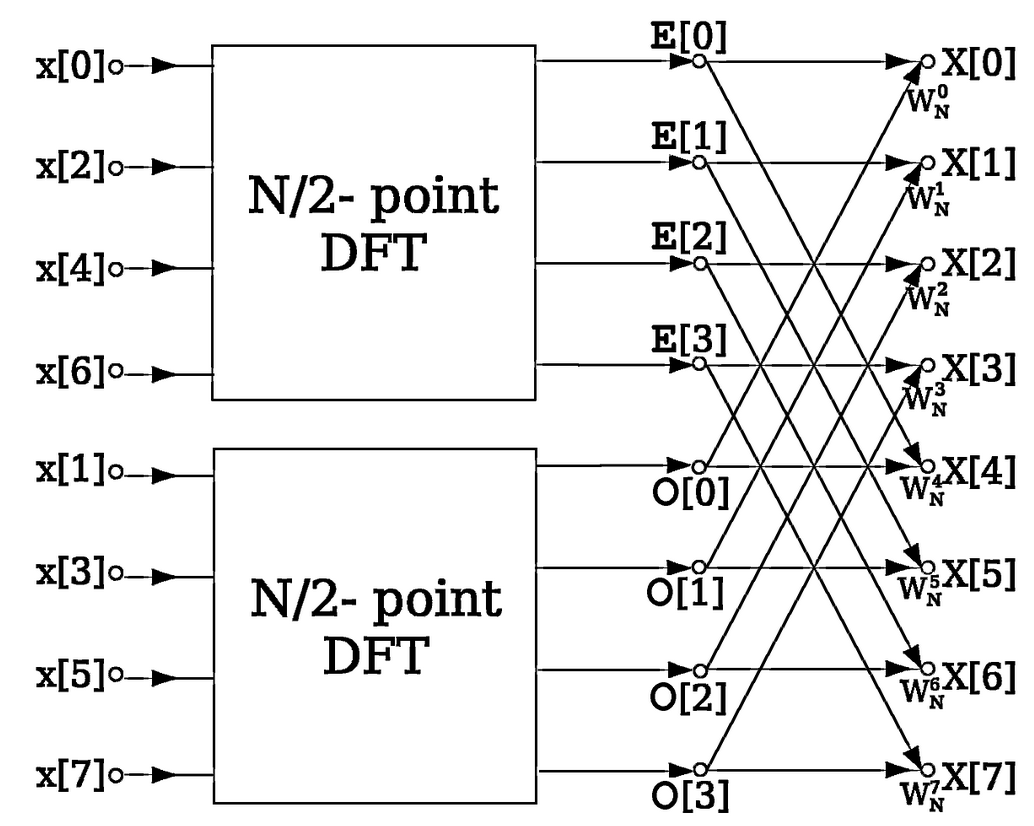
\includegraphics[width=10cm]{img/dft.png}
\caption{\label{fig:tsm}[AÑADIR LA FIGURA 1 Y 2 DEL PAPER EN LA MISMA IMAGEN]}
\end{center}
\end{figure}

En las propias palabras de los autores, la idea consiste en descartar y repetir algunos segmentos de la señal para comprimir o expandir la longitud del audio resultante. Utilizan para ello un sistema de buffer circular con dos punteros que se mueven a diferente velocidad pero con algunas variaciones para evitar que colisionen. En consecuencia, los saltos que realiza el puntero "rápido" tienen longitud variable y pueden ser en cualquier dirección, puesto que la distancia entre este y el otro puntero es variable. Además se calcula el mejor punto para realizar el salto mediate AMDF (ecuación \ref{eq:amdf} para evitar una discontinuidad demasiado abrupta que resulte percetible al oído. 

\begin{equation}
\label{eq:amdf}
D(m) =  \sum_{k = 0}^{L - 1}|~x(k+m)-x(k)~|
\end{equation}

La función AMDF se utiliza como alternativa al método de la autocorrelación para detectar la afinación de la nota dado un conjunto de muestras cuando la función es mínima sin tener que recurrir a Fourier. Cuando es mínima dentro del área de búsqueda, estamos en el punto de salto adecuado. 

En resumen, combina varias operativas para lograr un algoritmo versátil que se pueda ajustar al factor de octavación deseado con una calidad relativamente buena en todos. Sin embargo, para llevar a cabo la ejecución de este algoritmo es necesaria una adaptación compleja porque precisa de mucha capacidad de cálculo en cada instante, haciédolo poco deseable para la FPGA. La siguiente solución presentada propone un mismo concepto de cálculo sencillo repetido en muchas ocasiones, lo cual resulta mucho más deseable a la hora de introducirlo en la placa.

\subsubsection{Algortimo de baja latencia}
\label{rhilbert}

Para comprender la base de esta operativa, descrita en profundida en \cite{hilbert}, hay que diferenciar dos maneras de abordar la problemática a grandes rasgos ya que la nomenclatura induce a error:
\begin{itemize}
\item \textbf{Desplazamiento de tono: }o \emph{pitch shifting}, se basa en que cada frecuencia se \textbf{multiplica} por una constante. Este el caso de los algoritmos descritos antes que pretendían dividir todas las frecuencias entre 2.
\item \textbf{Desplazamiento de frecuencia: }o \emph{frequency shifting}, en este caso a cada frecuencia se le \textbf{suma} (o resta) una constante definida. Estas técnicas no se han aplicado anteriormente en algoritmos de cambios de afinación porque se rompen las relaciones armónicas entre una fundamental y sus componentes. Sin embargo, esta va a ser la solución que proponen los autores para construir el algoritmo de baja latencia.
\end{itemize}
De forma equivalente, si a cada frecuencia le restamos su frecuencia mitad, $f_{out} = f_{in}-f_{in}/2$, obtenemos también la división por 2. Para que esta idea funcione, haría falta \emph{fijar} las frecuencias entrantes de alguna manera, ya que si no, no podríamos saber a priori qué constante hay que utilizar en cada momento. La solución es utilizar un banco de filtros IIR lo suficientemente estrechos como para que se distingan correctamente dos notas sucesivas. De esta forma, se realiza la resta inmediatamente despues de haber hecho el filtrado, como se muestra en \ref{fig:fshil}. Conociendo la afinación del saxofón, se pueden conocer a priori las frecuencias de entrada, por lo que habrá que centrar cada filtro con una de las notas del registro. El restro del espectro correspondiente a los armónicos se cubre con filtros equiespaciados siempre en escala logarítmica.

\begin{figure}
\begin{center}
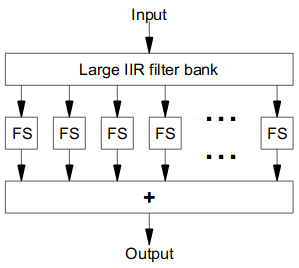
\includegraphics[width=5cm]{img/filtros_hilbert.png}
\caption{\label{fig:fshil}Esquema del algoritmo de baja latencia. FS es cada resta de frecuencia}
\end{center}
\end{figure}

Tal y como proponen los autores es necesario que el ancho de banda de cada filtro vaya aumentando con la frecuencia pero estableciendo un mínimo de 50Hz para las frecuencias más bajas. En esto radica uno de los problemas de este algoritmo y es que, produce inevitablemente una ligera desafinación que se puede acumular si se pierde la relación entera con los armónicos superiores. Esta desafinación es más pronunciada en las frecuencias inferiores debido al ancho de banda mínimo establecido ya que cada filtro coge una o dos notas.

Para realizar cada etapa de restado, son necesarios dos osciladores a 90º, una transformada de Hilbert y otros pocos componentes más, como ilustra la figura \ref{fig:restahil}. Adicionalmente, se puede sustituir la etapa de la transformada de Hilbert por filtros IIR, reduciendo aún más el coste computacional total. No obstante, es cierto que el elevado número de módulos, aunque sencillos, tienen un coste de área grande en la FPGA aunque no resulta crítico.

\begin{figure}[!tb]
\begin{center}
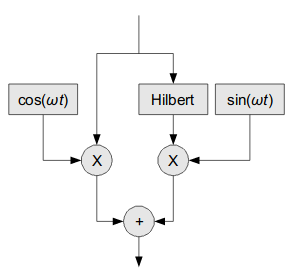
\includegraphics[width=5cm]{img/fs_hilbert.png}
\caption{\label{fig:restahil}Esquema de cada etapa de restado en el dominio del tiempo}
\end{center}
\end{figure}

La razón para no implementar este algoritmo de baja latencia ha sido puramente personal, ya que he priorizado eliminar el desafinamiento a reducir la latencia. En la fuente bibligráfica (\cite{hilbert}) hay muestras de audio de buena calidad comparando diferentes métodos, pero ninguno de ellos estaba implementado en FPGA. Es evidente que no se puede comparar de igual manera; las pérdidas que se producen debido al tratamiento de la señal muestra a muestra en la FPGA no se producen en un procesador. Dado que la implementación no va a ser óptima en ninguno de los casos, me ha resultado preferible implementar un algoritmo más sencillo que reduzca el número de puntos criticos en el mismo.

\subsection{Retorno a la transformada}
Así pues, se va a plantear una arquitectura basada en la idea del \emph{Vocoder de fase} que se presenta en los epígrafes sucesivos.
\section{Vocoder}
Durante todo el siglo XX se han ido desarrollando diferentes técnicas de tratamiento y codificación para la voz, conforme iba la tecnología en aumento. La consecuencia de ello es la aparición de diversos algoritmos que permiten este tipo de operaciones con una carga computacional relativamente baja. 

Un \emph{Vocoder}\footnote{Del inglés voice (voz) junto a encoder (codificador)} es generalemente cualquier aparato que analiza y/o sintetiza la voz humana para lograr  algún objetivo concreto, como compresión de datos, multiplexación o encriptación en la mayoría de los casos.

El Vocoder de canal\footnote{Del inglés "channel vocoder"}, desarrollado por los famosos \emph{Bell Labs} en 1928, utilizaba varios filtros multibanda seguidos por detectores de envolvente cuyas señales de control se transmitían al decodificador del receptor. Estas señales de control son mucho más lentas que la señal original a transmitir, por lo que se puede reducir el ancho de banda permitiendo a un mismo medio de transmisión soportar un mayor número de canales, ya sea por radio o cable. Finalmente, el decodificador amplifica estas señales de control y las introduce en los filtros correspondientes a cada banda para poder sintetizar de nuevo la señal original. Además de las ventajas sobre el ancho de banda, también se ayuda a proteger la señal para que no se pueda interceptar. Encriptando las señales de control y modificando los parámetros de los filtros, se puede hacer muy difícil su correcta reinterpretación si no se sincronizan el codificador y el decodificador. Esto popularizó su uso durante la Segunda Guerra Mundial en el bando aliado patentándose diversos diseños.

El concepto se ha mantenido contante durante todo el siglo hasta nuestros días, donde podemos ver implementaciones modernas de la misma idea, por lo que se ha desarrollado una estandarización. La voz humana posee un rango de frecuencias de entre 200 y 3400 Hz típicamente, por lo que se optó por una frecuencia de muestreo de 8 kHz. Es común que se utilice una codificación con 16 bit por muestra por analogía con el estandar CD, pero con utilizar al menos 12 la mayoría de los receptores será capaz reproducir la señal con una fidelidad razonable. Citando un ejemplo, los codificadores según la norma ITU G.729, que son utilizados en telefonía comercial, tienen una buenísima calidad con una tasa binaria de 8 kbps. Actualmente también se utilizan para desarrollar tecnologías relacionadas con la lingüistica, la física y la neurociencia.

\subsection{Vocoder en la música}
Paralelamente a su utilización en comunicaciones, el vocoder se comenzó a popularizar durante la década de los 70 como método de síntesis. Cabe mencionar, que durante esta década, surge un gran interés en los músicos por experimentar con diferentes timbres y sonidos en instrumentos conocidos o experimentales. Para aplicaciones musicales, se utiliza una frecuencia portadora proveniente de un instrumento en lugar de extraer la frecuencia fundamental del sonido que se esta grabando. El resultado es una deformación del sonido capturado que, por estar afinado en una nota adecuada, produce un resultado agradable al oído. Fue el primer fabricante de sintetizadores y pionero de la música electrónica, Robert Moog, el que desarrollo un prototipo llamado \emph{Farad} en 1968 pero no fue hasta 1970 cuando unieron el funcionamiento de esta máquina con el sintetizador modular \emph{Moog} que había lanzado previamente al mercado. Quedaba ya conformada la esencia de utilizar la señal proveniente de un micrófono como moduladora y la proveniente de sintetizador como portadora para modularla. Algunos ejemplos tempranos de músicos reconocidos  que utilizaron estos dispositivos fueron Phil Collins, Mike Oldfield, Stevie Wonder, Herbie Hancock o Michael Jackson.

\begin{figure}
\begin{center}
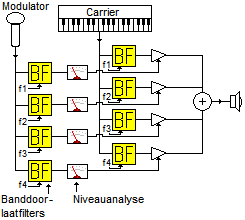
\includegraphics[width=7cm]{img/music_vocoder.png}
\caption{Esquema del funcionamiento de un vocoder musical}
\end{center}
\end{figure}

Estos vocoder proporcionaban sonidos a los que el público estaba poco acostumbrado pero que realmente no mantenían una fidelidad tímbrica respecto el sonido que captaban. Por ello se empezaron a utilizar los vocoder de fase los cuales permiten llevar a cabo expansión o compresión en el tiempo y \emph{Pitch Shifting}, es decir, modificar la altura musical del sonido o afinación sin cambiar la forma de onda que proporciona el timbre característico.

El método para hacerlo es el siguiente. En primer lugar se lleva a cabo una transformada mediante STFT (Short Time Fourier Transform) para posteriormente modificar la afinación mediante sub y sobremuestro. Este proceso hace que el audio resultante no resulte reconocible, por lo que es necesario ajustar el valor de la fase de cada muestra para mantener la coherencia entre ellas, de ahí el nombre de vocoder de fase. Una vez calculadas las muestras, se transforman de vuelta al dominio del tiempo, donde se rellena con ceros para obtener la misma duración que la señal entrante. A continuación se explican en detalle estas etapas.

\section{Transformación a frecuencia: STFT}

Una STFT se usa para determinar el módulo y fase de muestras próximas de una señal mientras cambia con el tiempo, haciéndola muy adecuada para aplicaciones en tiempo real. Para ello, se divide la señal en segmentos más cortos de la misma longitud y se calcula la transformada de Fourier de cada uno de ellos por separado. El método para calcular la transformada es indiferente pero al priorizar una baja latencia conviene decantarse por el algoritmo de la Transformada Rápida de Fourier o FFT.

\subsection{Transformada de Fourier: FFT e iFFT}

Para realizar la transformación al dominio de la frecuencia, la opción más adecuada es sin duda el algoritmo de la Transformada Rápida de Fourier o FFT\footnote{Del inglés Fast Fourier Transform}. Este algoritmo calcula la Transformada de Fourier en Tiempo Discreto o DFT\footnote{Del inglés Discrete Fourier Transform} descomponiendo la señal original de longitud $N$ en fragmentos de tamaño $N/2$ como muestra la figura~\ref{fig:fft} y posteriormente multiplicarlo por los términos $W_{n}$ calculados previamente. Nótese que en los bloques de $N/2$ se puede volver a aplicar el mismo principio de forma recursiva. Esto consigue reducir el tiempo de cálculo porque la transformada propiamente dicha se calcula para una longitud mucho menor. En la ecuación~\ref{eq:FFT} correspondiente la DFT genérica podemos ver como la complejidad depende cuadráticamente de la longitud de la entrada $O({n^{2}})$ mientras que la FFT lo realiza únicamente con $O({n*\log (n)})$.

\begin{figure}[!ht]
\begin{center}
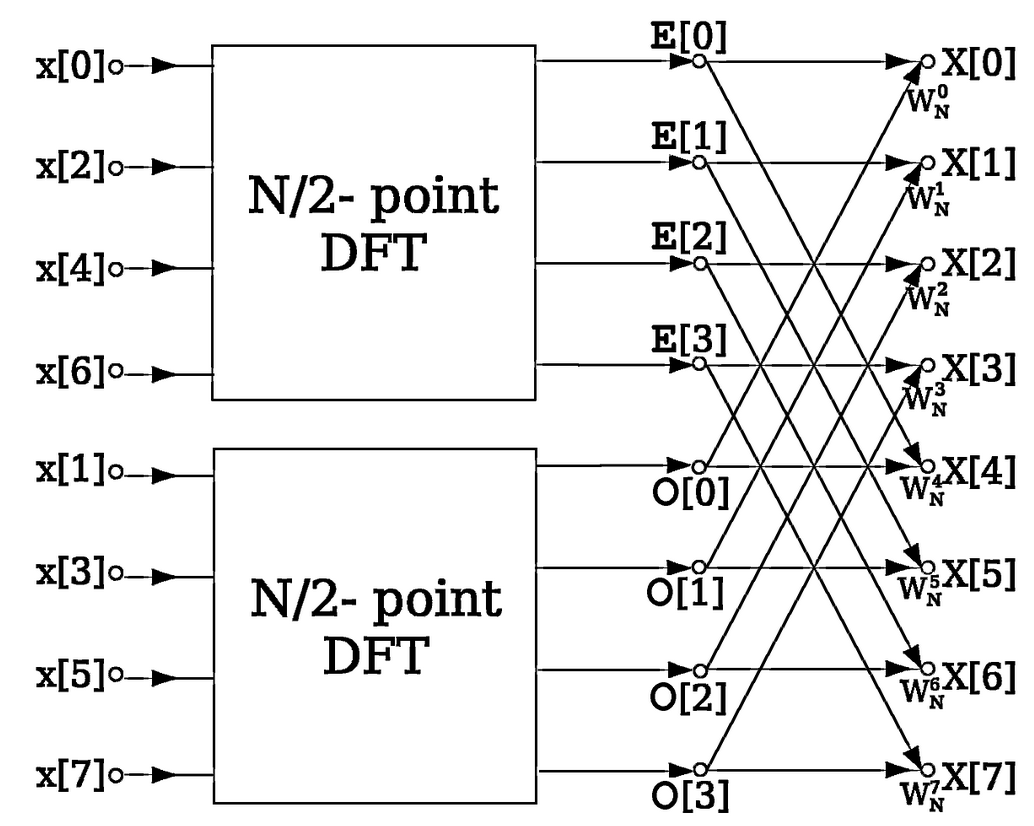
\includegraphics[width=10cm]{img/dft.png}
\caption{\label{fig:fft}Esquema del algoritmo para la realización de la FFT}
\end{center}
\end{figure}

\begin{equation}
\label{eq:FFT}
X(k) =  \sum_{n = 0}^{N - 1} x_{n}e^{-2\pi kni/N}~~~~~~~~Donde~~~~k = 0, 1...., N-1
\end{equation}
\begin{equation}
\label{eq:iFFT}
x(n) = \frac{1}{N} \sum_{n = 0}^{N - 1} X_{k}e^{-2\pi kni/N}~~~~~Donde~~~~n = 0, 1...., N-1
\end{equation}

El caso de la transformada inversa es totalmente análogo, el algoritmo de la FFT se puede aplicar de la misma forma para realizar iDFT de forma más rápida, lo que se conoce como iFFT. La ecuacion~\ref{eq:iFFT} muestra la expresión genérica de la iDFT para un señal de N muestras. Cada uno de los parámetros que se utilizan para realizar las transformaciones se encuentra explicado en el apartado de implementacion HACER LA CITA.

\subsection{Solapamiento y enventanado}

Dividir la señal entrante en sucesivas tramas es un proceso sencillo, únicamente se almacenan las muestras en una memoria para introducirlas posteriormente en el módulo que realiza la FFT. El problema entonces reside en la propia naturaleza de la FFT y es que esta funciona perfectamente para señales periódicas, pero al dividir la señal, no se garantiza que estas tramas contengan un número entero de periodos. Esto se agudiza especialmente cuando la señal es variante con el tiempo y el número de elementos por trama es independiente de la frecuencia de la señal de entrada.

\begin{figure}[!ht]
\begin{center}
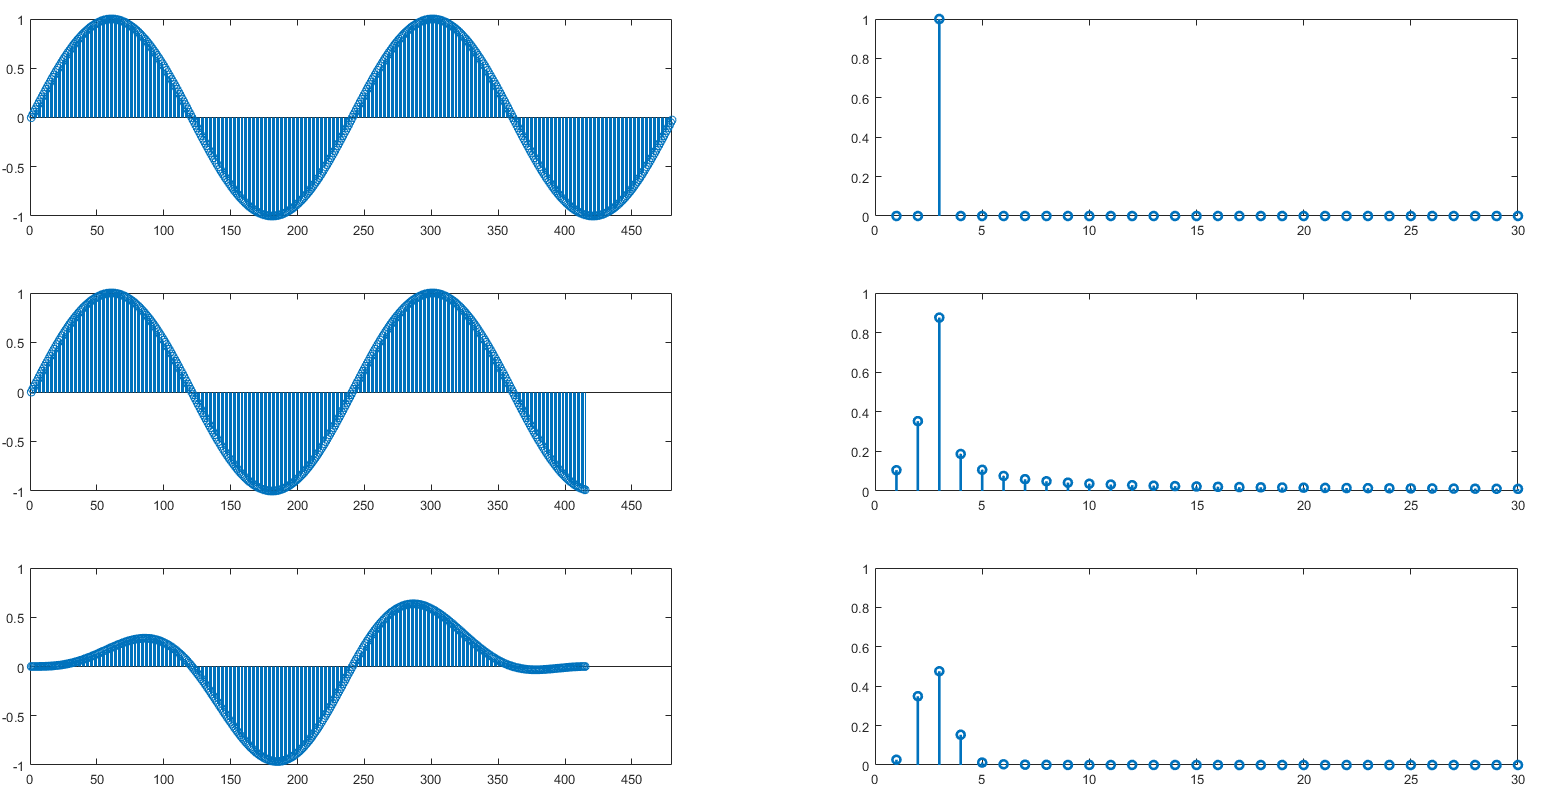
\includegraphics[width=14cm]{img/problem_fft.png}
\caption{\label{fig:probfft}Señal sinoidal y su FFT con periodos enteros, recortada y enventanada}
\end{center}
\end{figure}

En la figura~\ref{fig:probfft} se ilustra el problema del recortado arbitrario descrito y su clara mejora al aplicarle enventanado. Frente al caso ideal, el primero, el corte introduce componentes en otras frecuencias que se traducirán como un ruido molesto al final de cada trama, conocido en en inglés como \emph{clipping}, al escuchar la transformada inversa. Podemos comprobar como al aplicar una ventana a la señal de entrada, este se hace menor y afecta a menos muestras. Para este ejemplo se ha utilizado una ventana de Hann como la que se utilizará en el prototipo.

Junto al enventanado, se suele aplicar \emph{solapamiento}, es decir, en lugar de empezar a construir una trama a continuación de la anterior, la empezamos a llenar antes de que se haya acabado de llenar la trama anterior, repitiendo muestras. De esta forma, las tramas están enlazadas entre ellas evitando una discontinuidad abrupta.

Generalmente se cuantifica este proceso mediante un \emph{factor de solapamiento, fs,} expresado en tanto por ciento. Si una trama t de longitud $n = 100$ muestras tiene un solapamiento de 15\%, las primeras $n*15\% = 15$ muestras de t son idénticas a las 15 últimas de la trama anterior, t-1, y así sucesivamente.

\begin{figure}[!b]
\begin{center}
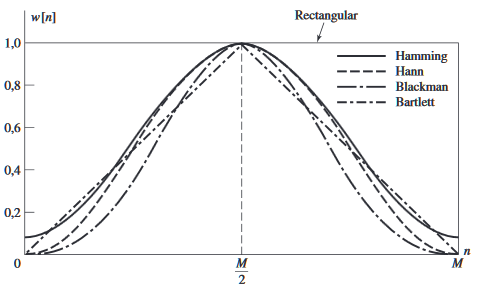
\includegraphics[width=10cm]{img/ventanas_grafica.png}
\caption{\label{fig:compven}Comparativa de las ventanas más utilizadas}
\end{center}
\end{figure}

Lógicamente, cuando aumentamos el factor de solapamiento más muestras procesamos y en consecuencia, menos eficiente es el algoritmo.Este desperdicio de recursos en el procesado supone un compromiso doble con las prestaciones. Por un lado, cuanto más disminuya esta eficiencia, más aumentará la latencia, ya que habrá que esperar al cálculo de la siguiente trama para poder finalizar la construcción de la trama presente. Por otro lado, resulta mucho más complejo de cara a la temporización en su implementación. 

Como conclusión, debemos elegir un factor de solapamiento $fs > 50$ para que resulte práctico, ya que si no el efecto es demasiado sutil para lo que supone su implementación. Tras un modelado en Matlab, he implementado finalmente un valor de $fs = 75\%$ tal y como recomienda Ellis~\cite{Ellis} en su implementación del vocoder de fase.

\begin{figure}[!b]
\begin{center}
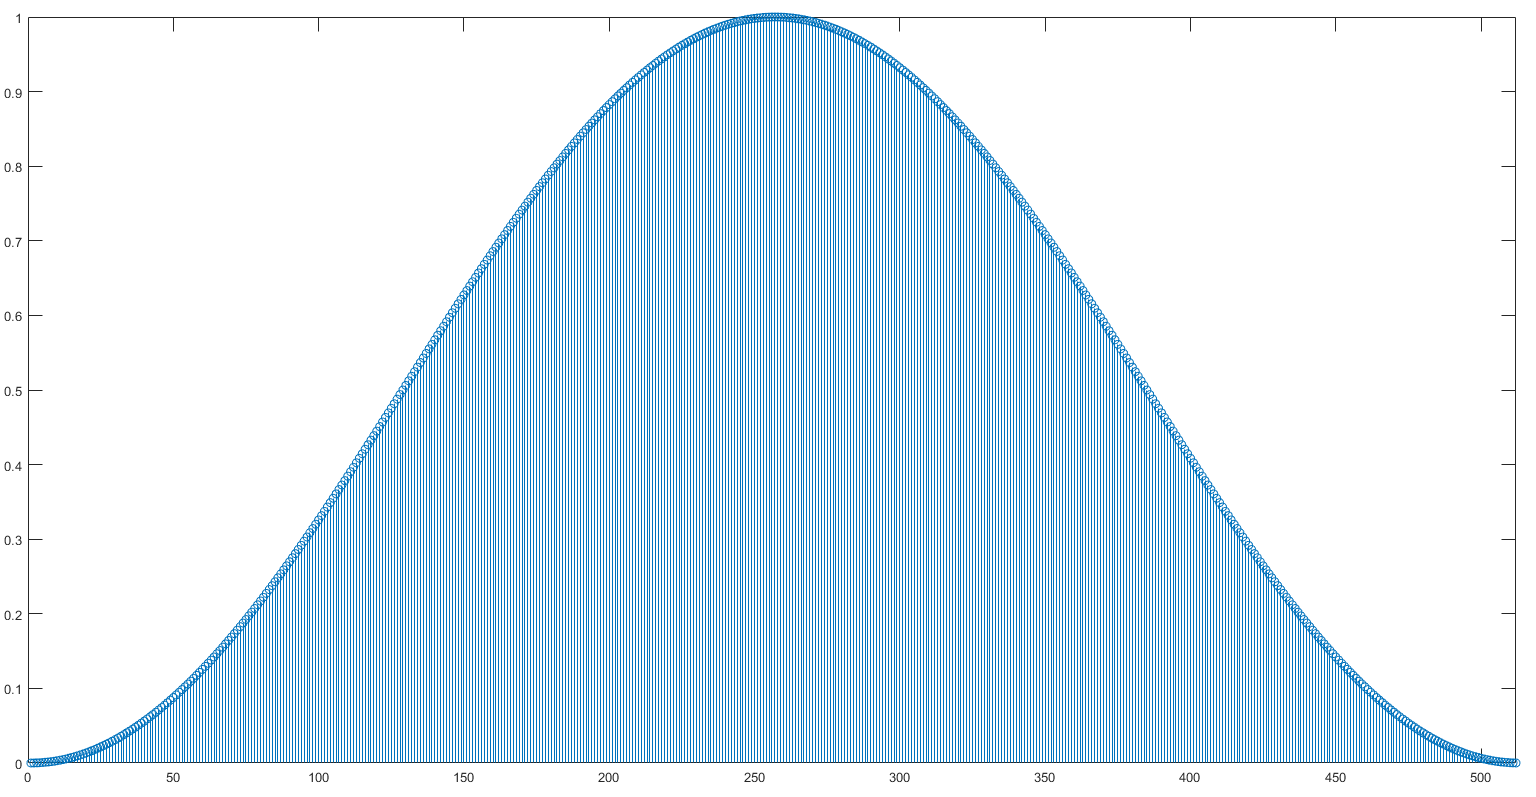
\includegraphics[width=15cm]{img/ventana_utilizada.png}
\caption{\label{fig:used_win}Ventana de Hann para $N = 512$ en Matlab}
\end{center}
\end{figure}

Como ya se ha visto antes, el solapamiento se utilizará junto con un enventanado de Hann cuya expresión se recoge en~\ref{eq:Hann}. Esta ecuación resulta sencilla de implementar y su uso está muy extendido para aplicaciones de audio en tiempo real frente a algunas de sus alternativas vistas en la figura~\ref{fig:compven}. El propio Ellis utiliza en su algoritmo~\cite{Ellis} una ventana de estas características.

\begin{equation}
\label{eq:Hann}
 H(n) = 0.5 * \left(1 - \cos\left(\frac{2\pi n}{N - 1}\right)\right)
 \end{equation} 
 
Estos mismos conceptos se utilizarán de forma completamente análoga en la etapa de la transformada inversa, tras introducir las muestras en el módulo iSTFT. La única excepción es que para mantener la amplitud de las muestras en la salida igual que las de la entrada, hay que aplicar un factor de escala de $2/3$. En la práctica, lo que se hará será realizar la multiplicación a las constantes de la ventana quedando una ventana de Hann donde cada muestra está escalada por el factor mencionado, ahorrando así una operación.

\section{Operaciones sobre la fase}
A grandes rasgos este algoritmo opera realizando un diezmado en frecuencia de factor 2, es decir, eliminando una de cada dos frecuencias entrantes, y posteriormente modifica la fase para evitar el desplazamiento circular mencionado en \ref{nofourier}. El procesado se realiza por \emph{tramas consecutivas pares}, dos tramas se agrupan para formar una pareja en la que se va a poder calcular el valor de una única trama de salida. De esta forma, la primera trama se agrupa con la segunda, la tercera con la cuarta y así sucesivamente.

\subsection{Cálculo del módulo}
El primer paso consiste en obtener el módulo de las muestras. Tras repasar el algoritmo, se puede ver que solo es necesaio calcular este valor para una de cada dos muestras, ya que la otra es la que será diezmada y por tanto, no merece la pena malgastar recursos en esta operación. 

El cálculo del módulo a partir de la forma binomial es sencillo: $mod = \sqrt{re^{2}+im^{2}}$ donde $re$ es la parte real e $im$ la imaginaria. Sin embargo, la implementación en FPGA de una raíz cuadrada no resulta inmediata. Una opción es utilizar un módulo de cálculo que procese los datos y devuelva la función raíz mientras que otra es utilizar $lookup tables$ para consultar el resultado de unas entradas previamente definidas. Este último método no es práctico ya que el tamaño de la memoria ROM que almacenaría esos datos tendría que ser demasiado grande, además el Vivado proporciona algunos módulos IP que realizan estas operaciones matemáticas, entre otras, a camibio de algunos ciclos de procesado.

En este caso, resulta más práctico realizar una aproximación que permita reducir el tamaño en área de la implementación así como la latencia de la misma, tal y como señala el doctor Chu en \cite{vhdlchu}. Si aproximamos por tanto según \ref{eq:mod_app}, $donde~x = max\{|a|,|b|\}, y = min\{|a|,|b|\}$, logramos simplificar en gran medida esta operación.

\begin{equation}
\label{eq:mod_app}
 \sqrt{a^{2}+b^{2}} \approx max\{((x - 0,125x) + 0,5y),x\}
\end{equation} 

\subsection{Recalculando la fase}
Una vez tenemos el módulo calculado, podemos calcular la nueva fase de cada muestra teniendo en cuenta una vez más que necesitamos la información de una trama $t$ y de la siguiente, $t+1$. El método para calcular la fase partiendo de la forma binomial es $\arctan(im/re)$ pero en este caso, si que compensa utilizar un core IP del Vivado que realice esta operación, ya que esta y otras operaciones trigonométricas serán necesarias más adelante.

Una vez calculada la fase de cada muestra entrante $n_{t}$, procedemos a obtener la fase de salida que se aplicará a cada muestra de salida $n_{t}'$. Primeramente calculamos una variable, $dp$, que va acumulándose con $n$ según \ref{eq:phcalc}. 
\begin{equation}
\label{eq:phcalc}
dp = fase(n_{t+1}) - fase(n_{t}) - dphi
\end{equation} 
En esta fórmula se puede observar la existencia de una constante $dphi$ de valor $dphi = (\frac{n\pi}{2})$\footnote{Esta $n$ también se refiere al número de muestra dentro de una trama $t$. Hay que recordar que $0 \leq n \leq puntos~de~la~transformada$, 511 en este caso} que se calcula aparte y se introduce en una ROM para utilizarla a lo largo del procesado. Aunque pueda parecer que el valor resultante puede llegar a ser muy elevado debido al carácter de esta constante, el siguiente paso es reducir el resultado obtenido al intervalo $(-\pi,\pi)$, eliminando el problema.

Esta constante $dp$ va a servir para actualizar el valor de la fase \textbf{de la muestra siguiente $n+1$} operando como en \ref{eq:phfin}, de forma que la fase de cada muestra depende de la anterior dentro de la misma trama.
\begin{equation}
\label{eq:phfin}
fase(n_{t}' + 1) = fase(n_{t}) + dp + dphi~~~~~~con~fase(n_{t}) = 0~~si~n=0
\end{equation} 
Tras este proceso, se puede preparar la muestra para iniciar la transformada inversa y posteriormente reenventanar la señal de salida cuando se procesen el resto de las muestras necesarias. [INCLUIR DIAGRAMA DE BLOQUES DE LA PARTE TRANSFORMADA]

Para concluir, podemos afirmar que el algoritmo que se va a implementar es una adaptación del vocoder de fase propuesto por Ellis (\cite{Ellis}), de forma que este orientado a la octavación y sea lo más adecuado posible para introducirlo en la FPGA.